\chapter{Methods}
\label{c:method}

In the following sections, first a number of typical RNA-Seq and DNA-Seq
pipelines that BioCloud supports are defined and explained. Then the design of
BioCloud is explained by breaking down into two main parts: the website and the
report generator. For the website, the components including account
registration, data sources management, experiment design, and pipeline
execution are described and their roles are illustracted in the website
overview workflow. For the report generator, the workflow demonstrates how
outputs are extracted, parsed, and rendered into pre-defined web-based report
templates.



\section{RNA-Seq pipelines}

The RNA-Seq analysis pipelines that BioCloud supports are summarized in
Figure~\ref{fig:dnaseq-pipeline}.

\begin{figure}[!htbp]
\centering
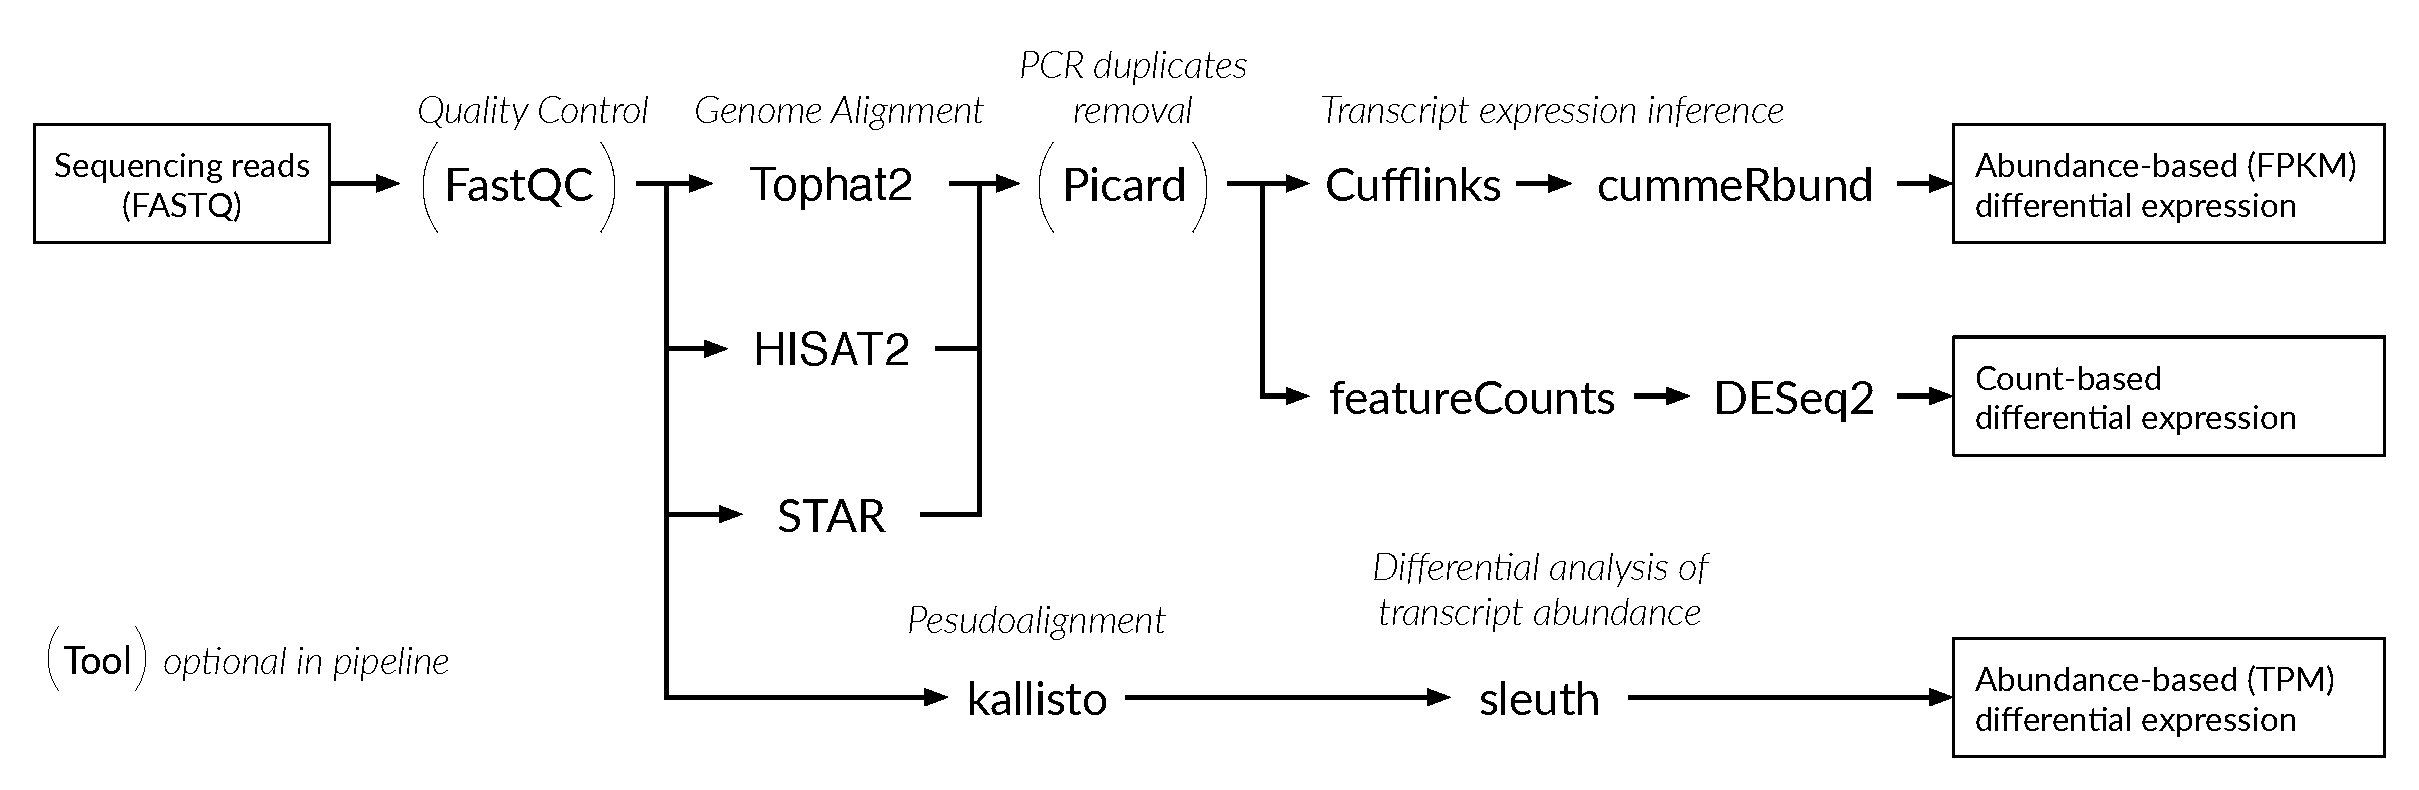
\includegraphics[width=\textwidth]{images/rnaseq_pipelines}
\caption[RNA-Seq analysis pipelines]{RNA-Seq analysis pipelines supported by BioCloud.}
\label{fig:rnaseq-pipeline}
\end{figure}



FastQC \cite{:fastqc}

Tophat2 \cite{kim2013:tophat2}

HISAT2 \cite{kim2015:hisat}

STAR \cite{dobin2013:star}

Picard \cite{:picard}

Cufflinks \cite{trapnell2010:transcript}

Cuffdiff \cite{trapnell2013:differential}

cummeRbund \cite{:cummerbund}

featureCounts \cite{liao2014:featurecounts}

DESeq2 \cite{love2014:moderated}

kallisto \cite{bray2016:nearoptimal}

sleuth \cite{pimentel2016:differential}


\section{DNA-Seq pipelines}

The DNA-Seq analysis pipelines that BioCloud supports are summarized in
Figure~\ref{fig:dnaseq-pipeline}.

\begin{figure}[!htbp]
\centering
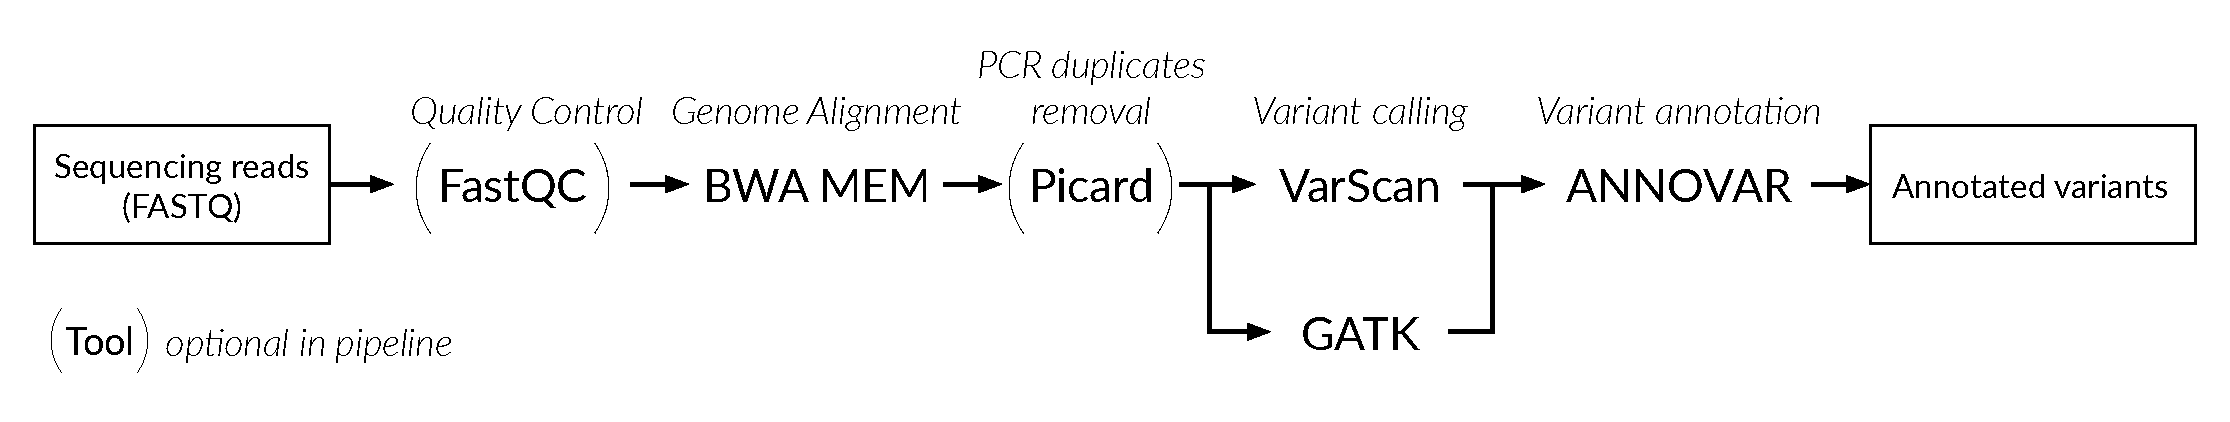
\includegraphics[width=\textwidth]{images/dnaseq_pipelines}
\caption[DNA-Seq analysis pipelines]{DNA-Seq analysis pipelines supported by BioCloud.}
\label{fig:dnaseq-pipeline}
\end{figure}




\section{Website workflow}

\begin{figure}[htbp]
\centering
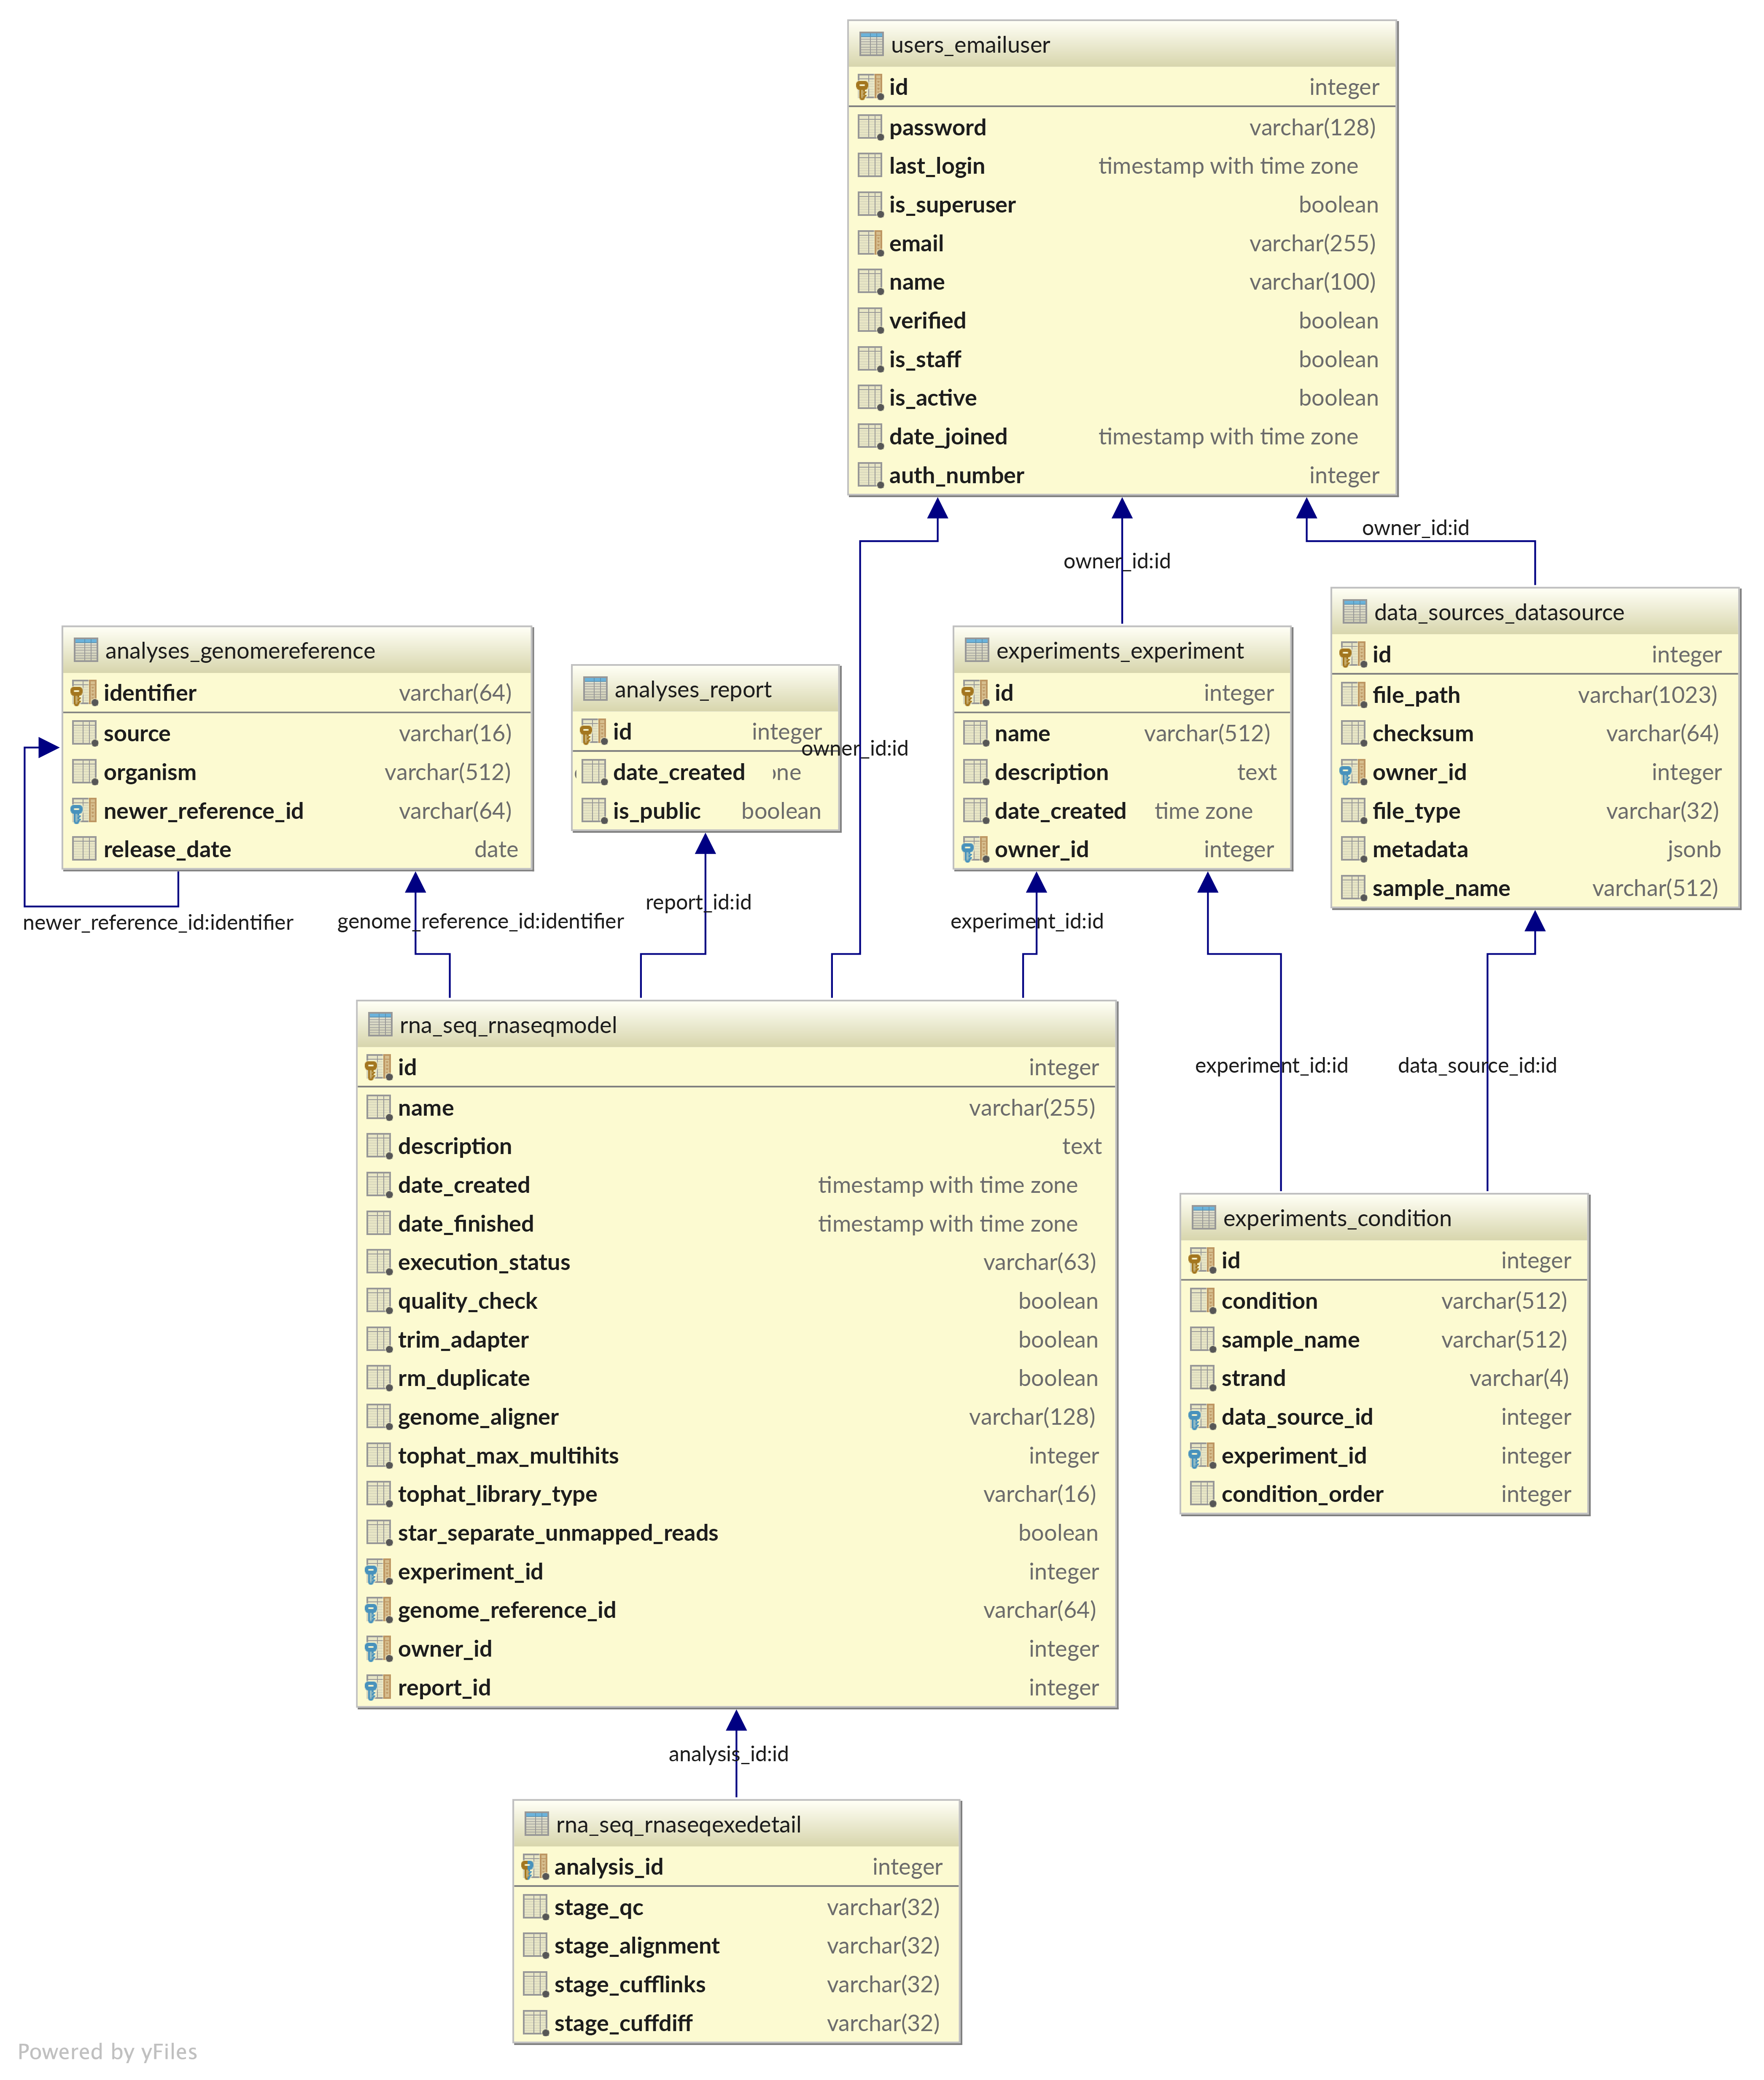
\includegraphics[width=\textwidth]{images/biocloud_erd}
\caption[Entity relation diagram (ERD) of BioCloud database]{
    Entity relation diagram (ERD) of BioCloud database. Here only one analysis
    pipeline of RNA-Seq (table \texttt{rna\_seq\_rnaseqmodel}) is shown for
    simplicity. Tables related with Django web framework internals and job
    queue framework are also omitted.
}
\label{fig:biocloud-erd}
\end{figure}


\subsection{Overall design}

\subsection{Message authentication and checksum}

Hash-based message authentication code (HMAC)

\subsection{HMAC-based account registration}

\subsection{Experiement design}

\subsection{Genome reference}

\subsection{Analysis submission}

\subsection{Job queue management}

\subsection{Report and result access control}



\section{Report generation}

\subsection{BCReport: result processing framework}



\section{Implementation}

\subsection{Website}

\subsection{Deployment}

\subsection{Report}
% vim: set textwidth=79:
